\section{Studienablauf}

Der Ablauf der Studie kann sich in drei Phasen untergliedern lassen: die Begrüßungsphase, die VR-Phase und die Abschlussphase. Im Folgenden wird der genaue Ablauf einer Durchführung der Studie beschrieben.

\subsubsection{Einleitungsphase}

Auf die allgemeine Begrüßung der Probanden folgte eine kurze Befragung zu den Erfahrungen mit VR und anderen Gaming-Medien. Dies war wichtig um daraufhin eine individuellere Erklärung der von uns verwendeten Geräte zu ermöglichen. 
Nachdem die Teilnehmer über die Ziele der Studie informiert wurden, erklärten wir ebenfalls die Funktionalitäten des Stuhls. Hierbei war es wichtig, dass Teilnehmer über die Einstellungsmöglichkeiten Bescheid wissen und dadurch eine möglichst entspannte Haltung einnehmen können. 
Anschließend wurden die Versuchsteilnehmer mit der VR-Brille vertraut gemacht. Im besonderen, wie sie die Brille für ihre Bedürfnisse entsprechend einzustellen haben und, falls der Proband ein Brillenträger war, was es noch zusätzlich zu beachten gibt.

Zusätzlich zur Einführung wurden den Probanden die üblichen Informationsbögen und eine Einverständniserklärung übergeben und die benötigten Unterschriften eingeholt. 

\begin{figure}[H]
	\centering
	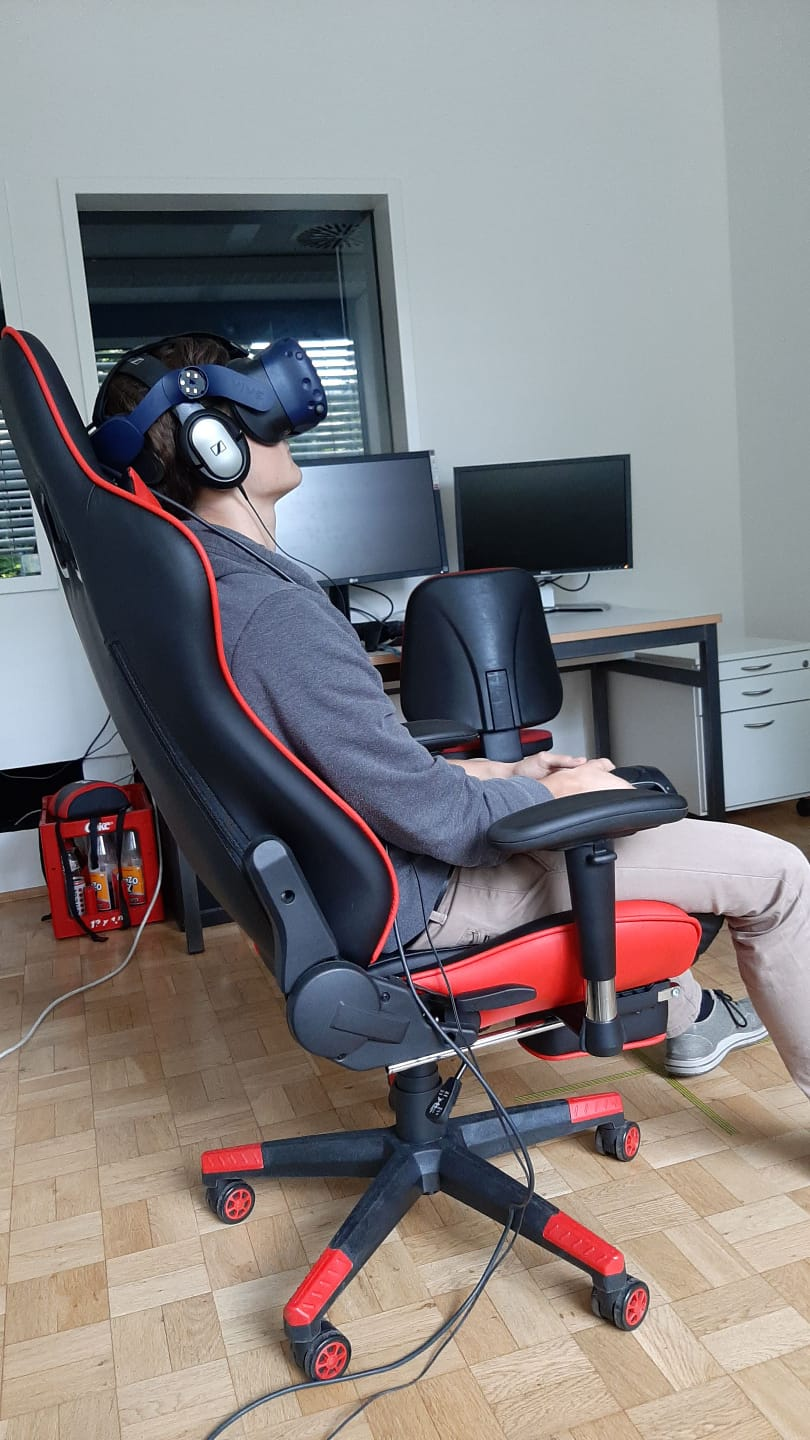
\includegraphics[width=0.6\textwidth]{./images/studie_awf.jpeg}
	\caption{Ein Proband beim Durchführen der Studie.}
	\label{fig:study_setup}
\end{figure}

\subsubsection{VR-Phase}

Die VR-Phase beginnt mir einer einführenden Erklärung der Umgebung und der Bedienung innerhalb dieser. Die Interaktion mit dem Trigger des Controllers lässt dem Nutzer einen Laser als Indikator erscheinen. 
Durch gleichzeitiges Zeigen und Betätigen des Triggers kann mit einzelnen Sphären innerhalb der VR-Umgebung interagiert werden.
Außerdem kann mit bekannten UI-Elementen aus anderen Programmen auf die gleiche Weise interagiert werden.
Diese Mechanik lässt sich vor der Ruhephase ausprobieren und sie stellt die grundlegende Mechanik dar, welche auch in den drei später folgenden Aufgaben von verwendet wird.

Nach dem Bestätigen der Instruktion wurde den Teilnehmern ein erster "`Self Assessment Manikin-Fragebogen"'~\cite{bradley1994measuring} (SAM) gezeigt. Die Auswahlmöglichkeiten für den Nutzer behandeln die Dimensionen Pleasure/Vergnügen, Arousal/Erregung und Dominance/Überlegenheit und die Symbolik ist in Abbildung~\ref{fig:sam_questionnaire} gezeigt.

\begin{figure}
	\centering
	\begin{subfigure}{0.5\textwidth}
		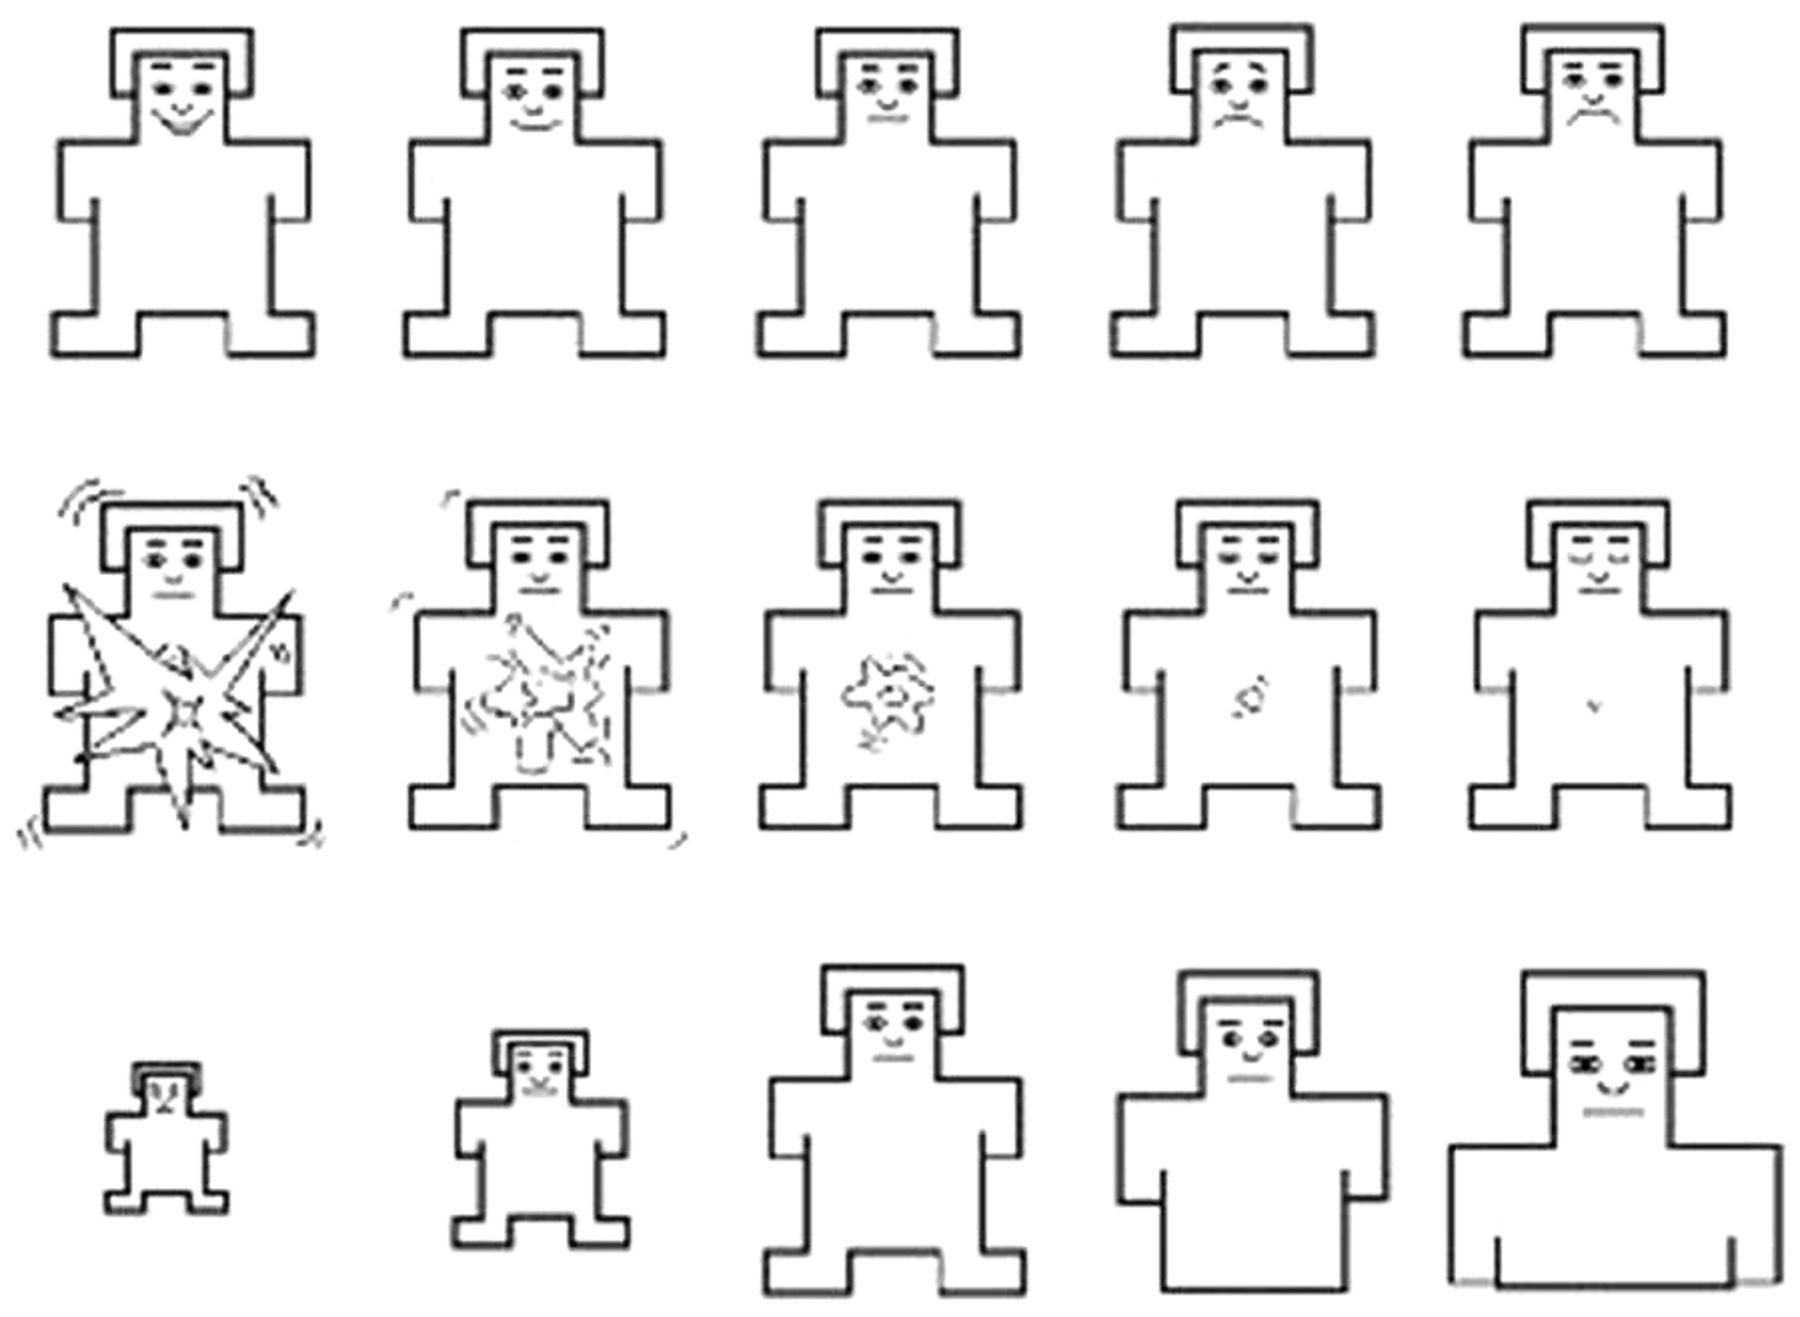
\includegraphics[width=\textwidth]{./images/F1_large.jpg}
		\caption{Self assessment manikin}
		\label{fig:sam_questionnaire}
	\end{subfigure}%
	\hfill
	\begin{subfigure}{0.25\textwidth}
		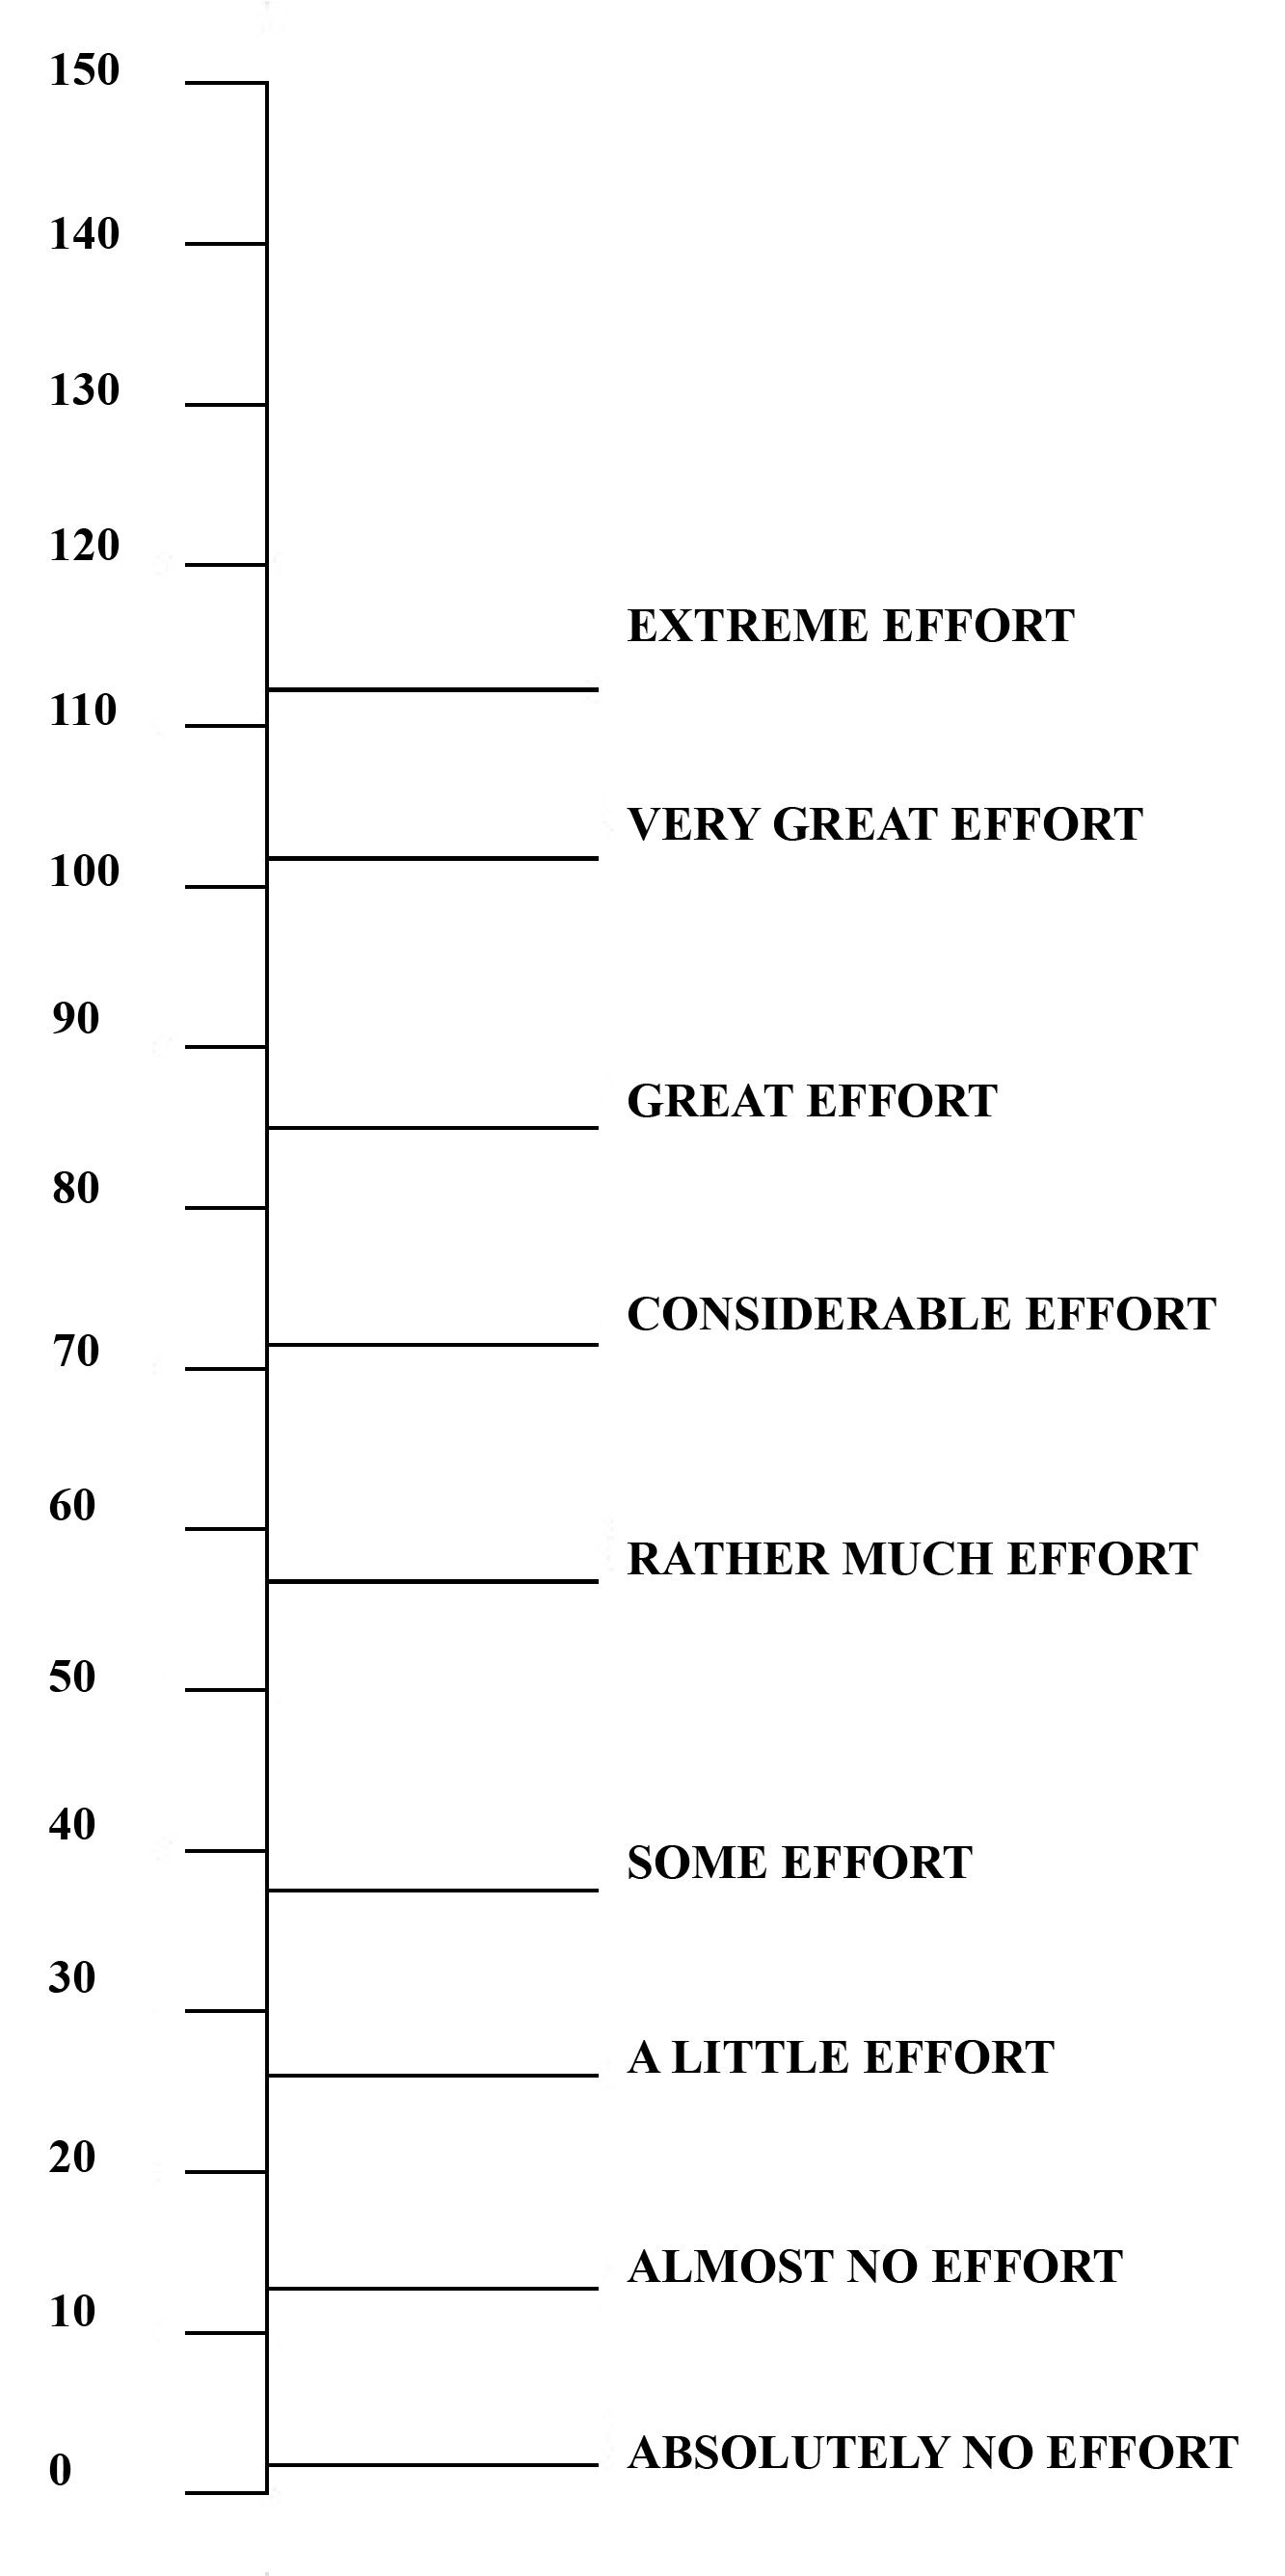
\includegraphics[width=\textwidth]{./images/rsme.png}
		\caption{Rating scale mental efford}
		\label{fig:rsme_questionnaire}
	\end{subfigure}
	\caption{Beispiele Self assessment manikin und rating scale mental efford.}
\end{figure}

Die Ruhephase beträgt bei jedem Probanden exakt 15 Minuten. Diese Information wurde den Teilnehmern allerdings vor der Studie nicht mitgeteilt.

Jeder Proband wurde innerhalb dieser Phase vom Studienbetreuer subjektiv beobachtet. Hierbei erfassten wir die Informationen zur Stuhleinstellung und ruhiges beziehungsweise unruhiges Verhalten innerhalb der VR-Umgebung. 
Letzteres wurde nach zehn Minuten der Ruhephase wiederholt wodurch zwei subjektive Parameter zur Aktivität des Teilnehmers entstanden. 
Bei der zweiten Aufzeichnung wurde der Fokus auf die Atmung des Versuchsteilnehmers gelegt.

Nach dem 'aufwecken' der Teilnehmer folgten die Aufgaben, welche in Abschnitt~\ref{sec:tasks} beschrieben wurden. Die Reihenfolge der einzelnen Aufgaben variierte hierbei nicht.

Sobald der Proband alle drei Aufgaben absolviert hat, wurde abermals der SAM-Fragebogen präsentiert. 
Zusätzlich hierzu wurde die Einschätzung der eigenen kognitiven Anstrengung mittels "`Rating Scale Mental Effort"' Fragebogen (RSME) abgefragt~\cite{wierwille1983validated}. Die Skala hierzu kann in Abbildung~\ref{fig:rsme_questionnaire} gesehen werden. 

Nach der Beantwortung aller Fragen in der VR-Umgebung endet die VR-Phase und das HMD kann abgenommen werden.

\subsubsection{Abschlussphase}

Nachdem der Hauptteil der Studie komplettiert wurde und das VR-Headset abgenommen werden konnte, mussten die Probanden noch eine demographischen Umfrage bearbeiten, welche diesmal nicht in VR stattfand, sondern an einem Computer im selben Raum. 
Dieser Fragebogen besteht zu Beginn aus allgemeinen, anonymen Fragen zur Person, Alter des Probanden, Geschlecht, gegebenenfalls der Studiengang, sowie ob der Proband schon vor der Studie Erfahrungen mit VR/AR gemacht hat. 
Anschließend musste der Versuchsteilnehmer Fragen zur Studie ausfüllen. Ob sich der Proband vor beziehungsweise nach der Studie müde gefühlt hat oder auch ob ein permanentes Tragen einer VR/AR-Brille vorstellbar wäre.
Nachdem dieser Fragebogen vollständig ausgefüllt wurde, befragten wir dir Teilnehmer noch nach ihrer Einschätzung zur Dauer der Ruhephase und notierten dies für Vergleiche. 
Zusätzlichen waren wir hier noch offen für allgemeine Anmerkungen ehe wir ihnen das Geld überreichten und sie verabschiedeten.
